\documentclass{beamer}
\usepackage[utf8]{inputenc}
  
\usetheme{Madrid}
\usecolortheme{default}
\usepackage{amsmath,amssymb,amsfonts,amsthm}
\usepackage{txfonts}
\usepackage{tkz-euclide}
\usepackage{listings}
\usepackage{adjustbox}
\usepackage{array}
\usepackage{tabularx}
\usepackage{gvv}
\usepackage{lmodern}
\usepackage{circuitikz}
\usepackage{tikz}
\usepackage{graphicx}
\usepackage[T1]{fontenc}
\UseRawInputEncoding

\setbeamertemplate{page number in head/foot}[totalframenumber]

\usepackage{tcolorbox}
\tcbuselibrary{minted,breakable,xparse,skins}



\definecolor{bg}{gray}{0.95}
\DeclareTCBListing{mintedbox}{O{}m!O{}}{%
  breakable=true,
  listing engine=minted,
  listing only,
  minted language=#2,
  minted style=default,
  minted options={%
    linenos,
    gobble=0,
    breaklines=true,
    breakafter=,,
    fontsize=\small,
    numbersep=8pt,
    #1},
  boxsep=0pt,
  left skip=0pt,
  right skip=0pt,
  left=25pt,
  right=0pt,
  top=3pt,
  bottom=3pt,
  arc=5pt,
  leftrule=0pt,
  rightrule=0pt,
  bottomrule=2pt,
  toprule=2pt,
  colback=bg,
  colframe=orange!70,
  enhanced,
  overlay={%
    \begin{tcbclipinterior}
    \fill[orange!20!white] (frame.south west) rectangle ([xshift=20pt]frame.north west);
    \end{tcbclipinterior}},
  #3,
}
\lstset{
    language=C,
    basicstyle=\ttfamily\small,
    keywordstyle=\color{blue},
    stringstyle=\color{orange},
    commentstyle=\color{green!60!black},
    numbers=left,
    numberstyle=\tiny\color{gray},
    breaklines=true,
    showstringspaces=false,
}



\title 
{MatGeo Assignment 4.13.76}

\author
{AI25BTECH11007}
\begin{document}

\frame{\titlepage}
\begin{frame}{Question}
    Two motorcycles A and B are running at a speed more than the allowed speed on
the road represented by the following lines:
\[
\mathbf{r} = \lambda(\mathbf{i} + 2\mathbf{j} - \mathbf{k}), \qquad
\mathbf{r} = (3\mathbf{i} + 3\mathbf{j}) + \mu(2\mathbf{i} + \mathbf{j} + \mathbf{k}).
\]

Based on the following information, answer the questions:

\begin{enumerate}
    \item Find the shortest distance between the given lines.
    \item Find a point at which the motorcycles may collide.
\end{enumerate}

\end{frame}

\begin{frame}{Solution}
    Let $\vec{x}_1$ and $\vec{x}_2$ be the points on the given lines respectively.
\[
\vec{x}_1 = \lambda\myvec{1\\2\\-1}, \qquad 
\vec{x}_2 = \myvec{3\\3\\0} + \mu\myvec{2\\1\\1}
\]

\textbf{(a) Shortest distance:}\\
Let $\vec{A} = \myvec{0\\0\\0}$ and $\vec{B} = \myvec{3\\3\\0}$

Let
\[
\vec{M} = \myvec{1 & 2 \\ 2 & 1 \\ -1 & 1}
\]

\begin{equation}
    (\vec{M} \, \, \vec{B}-\vec{A}) = \myvec{1 & 2 & 3 \\ 2 & 1 & 3 \\ -1 & 1 & 0}
\end{equation}

\end{frame}
\begin{frame}
Row Transformation-1: $R_2 \rightarrow R_2 - 2R_1$
\begin{equation}
\myvec{1 & 2 & 3 \\ 0 & -3 & -3 \\ -1 & 1 & 0}
\end{equation}

Row Transformation-2: $R_3 \rightarrow R_3 + R_1$
\begin{equation}
\myvec{1 & 2 & 3 \\ 0 & -3 & -3 \\ 0 & 3 & 3}
\end{equation}

Row Transformation-3: $R_3 \rightarrow R_3 + R_2$
\begin{equation}
\myvec{1 & 2 & 3 \\ 0 & -3 & -3 \\ 0 & 0 & 0}
\end{equation}

Therefore, \(\operatorname{rank}=2 < 3 \Rightarrow\) The Lines intersect (not skew).

\begin{align}
    \boxed{\text{The Shortest Distance between the given Lines = } 0 \text{ units}}
\end{align}
    
\end{frame}
\begin{frame}
\textbf{(b) Intersection Point:} 

At intersection, the points on the lines are equal:
\[
\vec{x}_1 = \vec{x}_2 \quad \Longrightarrow \quad
\lambda\myvec{1\\2\\-1} = \myvec{3\\3\\0} + \mu\myvec{2\\1\\1}
\]

Equating components gives a system of equations:
\[
\begin{cases}
\lambda - 2 \mu = 3 \\[1mm]
2 \lambda - \mu = 3 \\[1mm]
- \lambda - \mu = 0
\end{cases}
\]

Write in augmented matrix form:
\[
\left[\begin{array}{rr|r}
1 & -2 & 3 \\[1mm]
2 & -1 & 3 \\[1mm]
-1 & -1 & 0
\end{array}\right]
\]  
\end{frame}

\begin{frame}
Row Reduction-1 : $R_2 \rightarrow R_2 - 2 R_1$
\[
\left[\begin{array}{rr|r}
1 & -2 & 3 \\[1mm]
0 & 3 & -3 \\[1mm]
-1 & -1 & 0
\end{array}\right]
\]

Row Reduction-2 : $R_3 \rightarrow R_3 + R_1$
\[
\left[\begin{array}{rr|r}
1 & -2 & 3 \\[1mm]
0 & 3 & -3 \\[1mm]
0 & -3 & 3
\end{array}\right]
\]

Row Reduction-3 : $R_3 \rightarrow R_3 + R_2$
\[
\left[\begin{array}{rr|r}
1 & -2 & 3 \\[1mm]
0 & 3 & -3 \\[1mm]
0 & 0 & 0
\end{array}\right]
\]

From $R_2$: $3 \mu = -3 \implies \mu = -1$ \\
From $R_1$: $\lambda - 2(-1) = 3 \implies \lambda + 2 = 3 \implies \lambda = 1$
\end{frame}
\begin{frame}
    \[
\therefore \lambda = 1, \quad \mu = -1
\]

Intersection point:
\[
\vec{r} = \lambda \myvec{1\\2\\-1} = \myvec{1\\2\\-1}
\]

\[
\vec{r} = \myvec{3\\3\\0} + \mu \myvec{2\\1\\1} = \myvec{1\\2\\-1}
\]

\[
\boxed{\text{Intersection Point = } (1,\,2,\,-1)}
\]

\end{frame}


\begin{frame}{Plot}
    \begin{figure}
        \centering
        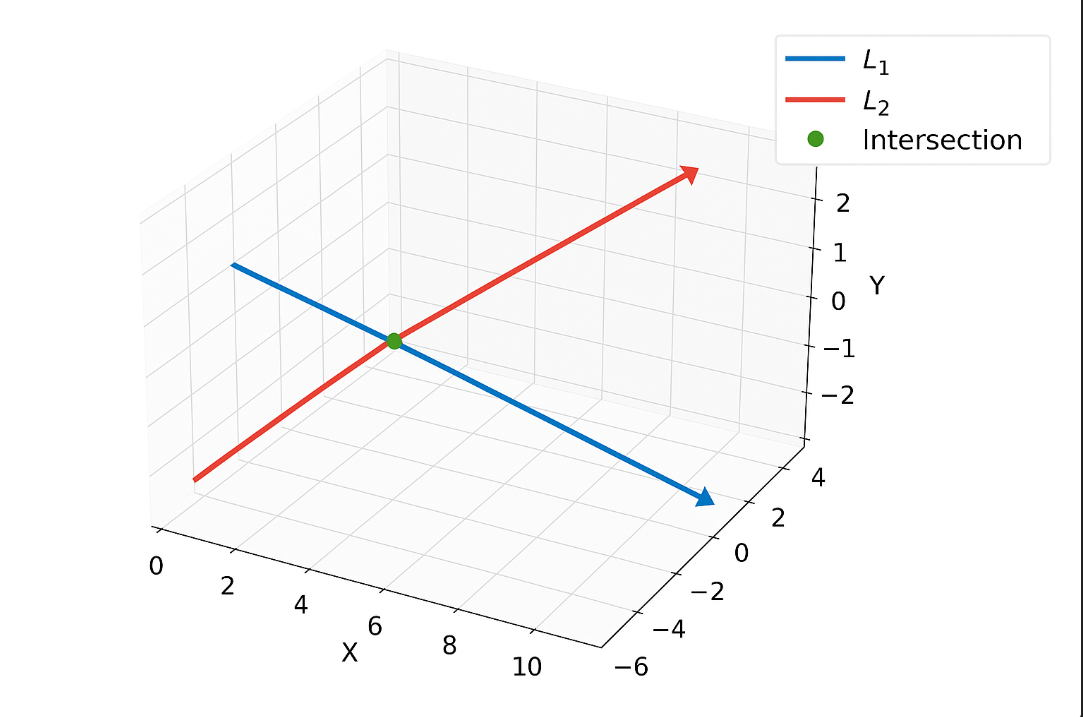
\includegraphics[width=0.75\linewidth]{figs/image.png}
        \caption{Image}
        \label{fig:placeholder}
    \end{figure}
\end{frame}

\begin{frame}[fragile]{C code}
    \begin{lstlisting}
        #include <stdio.h>

int main() {
    // Augmented matrix for the system
    // lambda - 2*mu = 3
    // 2*lambda - mu = 3
    // -lambda - mu = 0
    double a[3][3] = {
        {1, -2, 3},
        {2, -1, 3},
        {-1, -1, 0}
    };

    int n = 2; // number of unknowns: lambda and mu
    double x[2]; // solution array
    \end{lstlisting}
\end{frame}

\begin{frame}[fragile]{C code}
    \begin{lstlisting}
        // Gaussian elimination
    for(int i=0; i<n; i++) {
        // Make the diagonal element 1
        double diag = a[i][i];
        for(int j=i; j<=n; j++) {
            a[i][j] /= diag;
        }

        // Eliminate the current variable from rows below
        for(int k=i+1; k<n; k++) {
            double factor = a[k][i];
            for(int j=i; j<=n; j++) {
                a[k][j] -= factor * a[i][j];
            }
        }
    }
    \end{lstlisting}
\end{frame}

\begin{frame}[fragile]{C code}
    \begin{lstlisting}
    for(int i=n-1; i>=0; i--) {
        x[i] = a[i][n];
        for(int j=i+1; j<n; j++) {
            x[i] -= a[i][j] * x[j];
        }
    }
    double lambda = x[0];
    double mu = x[1];
    printf("Solution:\n");
    printf("lambda = %.2lf\n", lambda);
    printf("mu = %.2lf\n", mu);
    double r[3];
    r[0] = lambda * 1;      // lambda * (1)
    r[1] = lambda * 2;      // lambda * (2)
    r[2] = lambda * (-1);   // lambda * (-1)
    printf("Intersection Point: (%.2lf, %.2lf, %.2lf)\n", r[0], r[1], r[2]);
    printf("Shortest Distance = 0 units (lines intersect)\n");
    return 0;}
    \end{lstlisting}
\end{frame}

\begin{frame}[fragile]{Python code}
    \begin{lstlisting}
        import numpy as np
A = np.array([
    [1, -2, 3],
    [2, -1, 3],
    [-1, -1, 0]
], dtype=float)

# Number of unknowns
n = 2  # lambda and mu
# Perform Gaussian elimination manually
for i in range(n):
    # Make the diagonal element 1
    diag = A[i, i]
    A[i, i:] = A[i, i:] / diag
    # Eliminate the current variable from rows below
    for k in range(i+1, n):
        factor = A[k, i]
        A[k, i:] -= factor * A[i, i:]
    \end{lstlisting}
\end{frame}

\begin{frame}[fragile]{Python code}
    \begin{lstlisting}
        # Back substitution
x = np.zeros(n)
for i in range(n-1, -1, -1):
    x[i] = A[i, n] - np.dot(A[i, i+1:n], x[i+1:n])

lambda_val = x[0]
mu_val = x[1]

print(f"lambda = {lambda_val}")
print(f"mu = {mu_val}")

# Intersection point
r = np.array([lambda_val*1, lambda_val*2, lambda_val*(-1)])
print(f"Intersection Point: {r}")
print("Shortest Distance = 0 units (lines intersect)")
    \end{lstlisting}
\end{frame}

\end{document}